\part{Performance Analysis}

\chapter{Performance Analisys Introduction} \label{analysis-introduction}
\emph{"Every database vendor cites benchmark data that proves its database is the fastest, and each vendor chooses the benchmark test that presents its product in the most favorable light"}\cite{burleson}.

In this chapter we will introduce the database performance analysis' problem, and so we will discuss about how to measure the performance, how to understand who is the fastest and how to choose the best database depending on your needs. This preface is not specific to in-memory databases, but can be generalized for every DBMS.
	
	\section{Impartiality Problem}
The most important problem related to performance analysis, and benchmarking, is the validity, understood as impartiality, of the results. It's impossible to develop a benchmark which produces the same results obtained by real applications, and it's very hard to have the results similar to real performance too. Moreover every benchmark may produce valid results only for a small set of applications, and therefore there is the need to use different benchmarks. All these difficulties were emphasized by vendors who, with benchmarks wars and benchmarketing, complained for fake results, and consequently brought to a lack of trust in benchmarks. In this section we discuss about these difficulties, starting from a benchmark's definition until an analysis of the main differences in benchmarks which produce different results.

		\subsection{Benchmark Introduction}
Before starting all this discussion, it's necessary to explain the benchmark's meaning in computer science. The term benchmark refers to the act of running a program, or a set of programs, against an object in order to evaluate its performance, but it is also mostly used to represent the program or programs themselves. In this work we refer to software benchmarks run against database management systems. The main purpose of a benchmark is to compare the performance of different systems across different platforms. With the advance of computer architecture, it is become more difficult to evaluate system's performance only by reading its specifications. Therefore a suite of tests is developed to compare different architecture. This suite of tests, intended as validation suite, is also used to verify the correctness, the properties of a software. 

In particular benchmarks mimics specific workload giving a good measure of real world performance. But ideally a benchmark should substitute the application simulated only if it is unavailable, because only the real application can show real performance. Moreover when performance is critical, the only benchmark that matters is the inteded workload.

The benchmark's world is full of challenges starting from a benchmark development, to the interpretetion of the results. Famous benchmark tend to become useless after some time, because the vendors tune their products specifically for that benchmark. In addition most benchmarks focus only on the speed which is expressed in term of throughput, and forget many other important features. Moreover many server architectures degrade drastically near 100\% level of usage, and this is a problem which is not always taken into consideration. Some vendor may publish benchmarks at continuous at about 80\% usage, and, on the other hand, some other benchmark doesn't take this problem into account, and execute only tests at 100\% usage.
		
		\subsection{Benchmark History} \label{bench-history}
As already highlighted in the previous paragraph, with the advance of computer architecture the performance analisys became more difficult: it's not possible to evaluate a system only by reading its specifications. A computer program, a benchmark, simulating a specific workload, became a solution to this problem.

The first benchmarks were developed internally by each vendor to compare their database's performance against the competitors. But when these results were published, they weren't considered reliable, because there was an evident conflict of interest between the vendor and its database \cite{gray}. This problem was not solved by a benchmark pubblication by a third party, which usually brought to a benchmark war.
	
		\subsubsection{Benchmark Wars}
Also when benchmarks were published by third parties, or even by other competitors, the results were always discredited by losing vendors, who complained for the numbers, starting often a benchmark war. A benchmark war started when a loser of an important and visible benchmark reran it using specific enhancements for that particular test, making them get winning numbers. Then the opponent vendor again reran the test using better enhancements made by a "one-star" guru. And so on to "five-star" gurus. Every result so obtained by a benchmark could not be considered a valid result, firstly because the vendors themselves don't give any credit to the result, secondly because the result, with its relative numbers, changes too much frequently. 

		\subsubsection{Benchmarketing}
Benchmarketing is a variation of benchmark wars. Due to domain-specific benchmarks there was always a benchmark which rated a particular system the best. Such benchmarks may perform only a specific operation promoting one database instead than others. For example a test may execute only one type of transaction, or more reads than writes and therefore promote an in-memory database over a traditional DBMS. To summarize, a benchmark may simulate different scenarios favouring a particular database. Therefore each vendor promotes only the benchmarks which highlight the strengths of their product, trying to impose them as a standard. This leaded to a ploriferation of confuse benchmarks and didn't bring any benefit to the benchmark's reputation.

		\vspace{0.5cm}
Although these phenomenons were drastically reduced by the foundation of the Transaction Processing Performance Council (TPC) in 1988, they are still alive nowday.

		\subsection{Benchmark Differences} \label{categories}
It is now evident how hard is to understand which database is the fastest. Benchmarks cannot be properly used to analyze the performance of several databases and choose simply the best. Every benchmark has a bias, testing some particular aspect of database systems, such as writes, reads, transactions and so on. Moreover every benchmark operation can be implemented in different ways by the same database: creating a connection for every operation or using a connection pool; use different transaction isolation level; load the whole database in RAM or split it in different hard disk partition; etc. Furthermore the same benchmark, with the same implemention for every database, can show dissimilar results when it runs on different platforms (hardware and software).

All these differences are grouped by three categories:
\begin{enumerate}
	\item Test scenario: reads, writes, etc.
	\item Test implementation: there are different way to implement the same transaction.
	\item Execution platform.
\end{enumerate}
	
		\subsection{The Axiom}
By this reasoning comes out the axiom which will guide the following chapters, and the work behind this thesis:

\label{axiom} \emph{"There is not a slower or a faster database: databases are only slower or faster given a specific set of criteria in a given benchmark"}.

This sentence comes from an article by Bernt Johnsen \cite{Bernt}, who, in response to a benchmark comparing HSQL and Derby, stated that it's easy to make a benchmark, but it is always hard to communicate the meaning of the results. The interpretation depends on too many criteria, so that it's not easy to say which database is the fastest, unless specifying the set of criteria used in the benchmark.
	
		\section{Measures}\label{measures}
Even if we cannot state which database is the best by analyzing their performances on standard benchmarks, we can still measure other parameters that can be later interpreted to choose the database system which best fit our needs.

When choosing a database, the most important features to evaluate and compare are:

\begin{description}

	\item[Throughput]: is the number of transactions per second a database can sustain. This is the most important feature to consider when evaluating a database system. The most representative application scenario to understand the meaning of the throughput is an on-line transaction processing system. This kind of application requires the database to sustain a certain number of transactions per second, based on the number of users, and not every database can suite the needs of the application itself. Another example is real time applications: they require even higher throughput as well as very low latencies. Therefore it is crucial to understand if a certain database is suitable for an application in terms of transactions per second.
	
	\item[Latency/responsiveness]: is the time the database takes to execute a single transaction. This is the most important parameter in real application where the response time is a vital feature. In some case, where transactions are executed synchronizedly by a single user, latency can be measured as the inverse of throughput.
	
	\item[CPU load]: is the average percentage of the CPU processing time used by the database. It becomes an even more important parameter when the database is not the only service running on a server. CPU is a precious and limited resource, shared by all processes in a particular machine, and although database systems are usually deployed on dedicated servers, embedded databases live collated with the application that uses them. Many in-memory database 	don't even have a "stand aone" version and are mainly used as embedded db.
	
	\item[Disk I/O]: is the measure of the amount of data transferred to and from the disk. It is often a bottleneck for every traditional databases. Altought pure in-memory databases never access to the disk, when adding durability through a transaction log file, disk I/O is a bottleneck for IMDBs too. This parameter could be considered less important since all databases will incure in the same performance bottleneck, but it is possible that different DB coudl use the disk in different ways and suffer more or less impacts from it.
	
	\item[File size]: is the size of the database image on the hard disk. While traditional DBMS' store objects (tables), indexes and a transaction log file on the file system, in-memory databases usually store only a journal file containing all the transaction executed on the database. Altought this may seem a small file, it can become very huge, even more than the database image. This measure is interesting whereas each database use different data structures.
	
	\item[RAM usage]: is the quantity of RAM a process uses while running. Talking about in-memory database, this can be another way to measure the size of the database image. In addition, this is a critical value to take in mind: IMDBs only works correctly and efficiently under the hypothesis that the RAM is enough to contain the whole database. Therefore this can be an important parameter to take into consideration when deciding if a DBMS fits your requirements.
		
	\item[Startup time] is the time the database needs to become operational. This is a very important parameters for applications which need high availability, and in this case the startup time plays a crucial role to respect the maximum time the application can be off-line or not completely operative. 
	
	\item[Shutdown time] is the time the database takes to shut down and kill the process.
	
\end{description}
	
	\section{Choosing a Database}
From the previous sections, it's now clear how difficult it is to use benchmarks to prove which database is the fastest. Even with a fair benchmark, which can be very useful to understand the performance of databases, it is still difficult to choose a database: performance is only one factor to consider when evaluating a database \cite{burleson}. 

Other factors to consider are:
\begin{itemize}
	\item The cost of ownership.
	\item The availability of trained DBAs.
	\item The vendor's technical support.	
	\item The hardware on which the database will be deployed.
	\item The operating system which will support the database.
\end{itemize}

In other words, it is very difficult to choose the right database for our needs, and, of course, while evaluating databases and benchmarks there is absolutely \emph{no winner}.

For this reason, what we will introduce in the next chapter is a suite of tests which has been developed with these concepts in mind. What we tries to achieve is a way for people to judge, analyze, verify and evaluate any DBMS (especially in-memory databases) with a chance of developing their own set of test and run the test suite on any hardware and under (virtaully) any operating system. The application is Java-based and so it ansures the widest coverage of both hardware and operating systems.


\chapter{Test Suite} \label{test-suite}	
In this chapter we are going to discuss the first of the three big differences, described in paragraph \ref{categories}, which make a database seem faster or slower: the test scenarios used to run a benchmark and to analyze database's performance. Besides a tests' description, a suite of test will be created, allowing us to analyze the databases' features of our interest. 

The tests are divided into three categories: base test case, load test case and acid test case. The first category contains simple tests configured as a race between databases, and it is used to obtain an approximate idea in an early stage. Instead, the second category simulate real application scenario, and it can give us a detailed analysis of the real database's performance. Finally the last category is built to understand if the database is ACID compliant.


	\section{Why Define Test Scenarios}
The axiom, previously described in paragraph \ref{axiom} at page \pageref{axiom}, expresses clearly the difficulty to analyze databases' performance and how every result obtained in a given benchmark depends on the specific set of criteria used in the benchmark itself. In paragraph \ref{categories} there is also a description of the three major categories in which the criteria fall. The first of these categories is test scenarios: different test scenarios may show completely different performance results. It's not possible to avoid this behavior, but we can define clearly every tests so that we will be aware of the differences between them. 

Moreover we can model these tests in a way they simulate real application scenarios, so that real performances will be very close to the results obtained by the tests.

	\section{Base Test Case}
Base test case is a collection of very simple tests, which are configured mostly as a race. This is exactly what the major part of benchmarks does, particularly Poleposition \cite{poleposition}.

Every test can execute different read/write operations on the database and all these operations are inside a loop. The word \emph{transaction}, used extensively in the following paragraphs, refers to an execution of the loop, and therefore all the operations inside it.

The key features of these kind of test are:
\begin{itemize}
	\item A fixed number of transaction before the test stop: so tests are configured as a race where every database must execute a certain number of transaction.
	\item A fixed amount of time before the test stop: as an alternative to a fixed number of transaction, every test run for a specific amount of time, executing the maximum number of transactions per second. 
	\item Different kind of object: tests must be able to create/retrieve/update/delete simple flat objects with few fields, or complex flat objects with many fields, or still hierarchical objects, and so on. This feature let us test effectively the performance on the objects used in the domain of our interest.
	\item Single task: to keep these test simple it's better avoid concurrent test, but it is still possible to implement concurrently the different operation executed on the database.
\end{itemize}
	
		\subsection{Race Test: Timed}
We already said base tests are configured inherently as a race. These tests can be used to show the maximum throughput the database can reach doing a particular operation on a specific object. Metaphorically it's like a rocket car in the desert trying to reach its speed limit. In a real application this is rarely useful, but can give us an idea of database's limits. 

In order to create a test scenario we have to define the object/s involved by the test, the operations on which the test loop and when the test should stop. For example:
\begin{itemize}
	\item The object represent a person, with only two fields: an id number and a name. This is a simple flat object. 
	\item The only operation executed by the test is a write operation: every time an object will be added to the database.
	\item 60 seconds is the stop condition of the test: after 60 seconds of execution of writes (objects person inserted in the database) the test stops.
\end{itemize}
Clearly the time is not a significant measure, every test's execution run for the same amount of time: 60 seconds. Instead of the time, a more interesting measure to take is the throughput. This test shows the maximum theoretical value for the throughput, which in a real usage scenario will never be outperformed. 

This test, and its results, are not useful to understand the real performance and potentiality of the database and so to choose the database for our needs, but it can be used in an early stage to reduce the databases' set which will be analyzed extensively with further tests. In other words we can throw away every databases whose maximum throughput is not enough to our needs.

		\subsection{Race Test: Transactions}
This test is really similar to the previous test. The only difference is in the stop condition:
\begin{itemize}
	\item The object represent a person, with only two fields: an id number and a name. This is a simple flat object (same as before). 
	\item The only operation executed by the test is a write operation: every time an object will be added to the database (same as before).
	\item 1.000.000 of transactions is the stop condition of the test: when 1.000.000 of writes are executed (objects person inserted in the database) the test stops.
\end{itemize}
While in the previous test the duration was meaningless, this time, like in a race, it shows which database is the fastest (the winner of the race). Despite this, the duration is still of little use. Also for the throughput the same considerations made before are still valid.

But this new test is useful also to take other interesting measures, such as the file size, whose meaning has already been exaplined in paragraph \ref{measures}. We can evaluate how the file size increase with the number of objects (person) inserted in the database. This is because, differently to the previous one, every test's execution perform a fixed amount of transactions. 

	\section{Load Test Case} \label{load-test-case}
Restrictions introduced by base tests are very evident although they can be useful in certain situation and for simple and fast approximate results. These restrictions are due to the impossibility to simulate real complex application scenario. Substantially the main restrictions are two:
\begin{enumerate}
	\item Real application scenario are rarely single thread/task: to stick to the axiom at paragraph \ref{axiom}, the best way to understand which database fits our needs is to make test scnerios most realistic as possible.
	\item The second restriction result from the first:trying to make test scenarios more realistic, it is necessary to introduce some sort of control for the throughput. When a test stress the database engine to its maximum level, some other mechanisms may not work properly, such as the garbage collector, caching, indexing, etc. In addition, when a test concurrently accesses the database, this restriction is even more evident: if a thread is not limited in its transactions per second, it may lower the performance of other threads.
\end{enumerate}

Base test case offer very important and useful results, but when the need to test the average load of a real application of our interest, they are not enough. These restrictions are solved by load test case, which allow a better simulation of the application scenario. The key features of these tests, differently by base tests, are:
\begin{itemize}
	\item Multi task: there will be not only a combination of read/write/update/delete in one transaction executed synchronizedly, but in more transactions running concurrently against the database.
	\item A bond on the throughput: for every transaction it is possible to specify the maximum throughput, if the database can reach it, in order to simulate real application usage.
\end{itemize}

From these features comes the name "load test case", which means the simulation of an average, or specific, load on a certain database. This idea, and the need of this kind of tests,  can simply be exaplined by a Bernt's metaphor, who has been already cited for the axiom at paragraph \ref{axiom}. The metaphor is:

\emph{"I don't buy the fastest car in the market. I don't even buy the fastest car I can afford. I buy a car I can afford that fits my needs... e.g. drive to the northern Norway with 2 grown-ups, 3 kids, a kayak, sleeping bags, a large tent, glacier climbing equipment, food, clothes and so on. Can't do that with a Lamborghini"}\cite{Bernt}.

This metaphor explain exactly the need not for the fastest database, but for a database which can sustain the load of the application without any complexity during its normal functioning, such as a database snapshot freezing all writes operation, or a bug/memory leak making the database crash.

		\subsection{Real Time Prepaid System}
Keeping these features in mind, we want to create a load test case to analyze exactly which performance  a database system  offers for a practical use case: a real time prepaid system, such as a telephone company. Basically the test is the concurrent execution of 3 different task, each involving complex transactions: check balance, accounts handling, and manage calls and services. 

We start describing the domain objects used by this test, and the we pass to analyze the three different task involved.
		
			\subsubsection{Domain Objects}
Domain objects involved by this test are typical for a telephone company who handle telephone calls for every person, which is rappresented by an account, and which can access to many service through a web application, offered by the company for its customers. There are four domain objects used byt this test:
\begin{description}
	\item[Account]: this object represent a customer in the real time prepaid system. It contains all the typical information needed by a telephone company, such as the balance, the type of subscription, etc. In other words, this is a complex flat object, that is having many private field but no hierarchies. In a real application there are millions of accounts instantiated in the database, one for every customer. This dimesion is also very important to make the simulation as real as possible, in order to get realistic results.
	\item[Msisdn]: it is the unique number which identify a subscription is a GSM or UMTS mobile network, it is the telephone number. Each msisdn object is linked to an account. Therefore there are also millions of msisdn objects in the database, referring to a real application.
	\item[Webuser]: this represents the customer logged in the company web site. It contains the username and the password to access to web services. In common with msisdn, it is linked to an account too, and both are simple flat objects: a very simple object with few fields.
	\item[Session]: when a customer start a call, an object session is created, and it keep all the information about the call which is going on, until the call ends. After the call this object doesn't is deleted. A session contain the start time of the call represented, and the time of the last unit. Each session references to an account, which started the call. But there are not as many sessions as accounts, not everyone will start a call in the same time, except New Year's Day!
\end{description}

			\subsubsection{Check Balance Task}
This task simulate a customer checking his residual balance for the prepaid card, a SIM in the case of the telephone company. First, the customer logins in the website or calls the dedicated number, and then read/listen his balance.

Each task, as already explained, corresponds to a transaction composed by different operations. This leads to illustrate how the task work in terms of operations executed:
\begin{enumerate}
	\item \emph{Read} randomly the msisdn if the customer makes a call or the webuser if he access to the website.
	\item \emph{Read} the account referenced by the msisdn or webuser, and then check the residual balance, a simple account's field.
\end{enumerate}
So this task executes a total of two read for every transaction.

Another important parameter to make this task a part of a load test is the amount of transactions per second this task should sustain. The average throughput for check balance task, considering there are millions of accounts in the database, is about ten transactions per second.

			\subsubsection{Accounts Handling Task}
The account handling task simulates the creation of a new subscription by a customer, and so the creation of the account object, and after the relative msisdn and webuser. 

The operations involved by this task are:
\begin{enumerate}
	\item \emph{Write} of a new account: all informations of a customer are inserted in the system by creating a new account object.
	\item \emph{Write} of a new msisdn, containing the telephone number of the new subscription.
	\item \emph{Write} of a new webuser with username and password for the customer.
\end{enumerate}
To sum up, this task executes three write on the database for every transaction.

To simulate a real scenario, the average throughput is about ten transactions per second.

			\subsubsection{Manage Calls and Services Task}
This task simulates a call started by a customer. After checking the balance, and therefore if the account is allowed to start a call or use a service, a new session is created and updated every 30 seconds, the unit time. On the average a call lasts about two minutes. After this time the session is deleted.

In terms of operations executed on the database, it can be described as follow:
\begin{enumerate}
	\item \emph{Read} the msisdn of the customer starting the call.
	\item \emph{Read} the account referenced by the msisdn, and its residual balance, and the other parameters, to check the user's permissions for the service requested.
	\item \emph{Write} a new object session and \emph{update} account's balance.
	\item \emph{Update} the session every 30 seconds and the account's balance.
	\item \emph{Delete} the session after the call is ended.
\end{enumerate}

This is the most complex and important task, because it represents a very frequent task. No wonder if the average throughput is about 2000 transactions per second.

			\subsubsection{Real Time Prepaid System Summary}
To sum up this whole load test we have to define the objects used by the test, the task concurrently executed, and when the test stop.

There are four domain objects involved by this test. Three of these are simple flat objects: msisdn, webuser and session. The forth is a complex flat object: account. The number of objects already initialized in the database, before the test start, is on the order of millions.

Three task are executed concurrently. One is the major task, simulating a customer's call, and it runs 2000 times per second. This task is the bottleneck of a real application, and it could be also tested alone in a base test to understand the database's limits in running this task, and therefore to have an idea of the database potentiality. The other two are minor task, in fact the throughput is limited to ten transactions per second.

This test is a load test and therefore we are not interested in stopping it after a certain amount of transactions executed. But what we want is to let the test run for many minutes until to many hours to understand if the database can sustain the load generated by the test. Then the stop condition will be a specific amount of time.
			
	\section{Acid Test Case}
Base and load test case are used to analyze databases' performance, but, as already said, a database is not made only by performance: there are many other parameters to take into consideration before judging a database, such as ACID properties. To make these tests an all-round test suite, we could add some tests for verifying databases' ACID properties. The above corresponds to the work done by the Transaction Processing Performance Council with their TPC-C benchmark \cite{TPC-C}: performance is not the only benchmark's goal, but ACID properties are tested too.

Especially the durability property is most interesting to analyze when talking about in-memory databases. Pure IMDB have no durability at all, while it can be added in different degree, as already described in paragraph \ref{durability}. Therefore would be very useful to know, except the vendor's words, how strong is the durability solution implemented by the in-memory database.

Nevertheless, testing ACID properties is not a simple goal to achieve. Particularly the durability is the hardest property to be tested. Also the tests developed by TPC are not intended to be an \emph{exhaustive quality assurance test}.
%Citazione tpc pdf pagina 46 \cite{TPC-C}

\chapter{Database Benchmark Softwares Overview}
The difficulty to analyze objectively databases' performance has already been exapalined and understood in chapter \ref{analysis-introduction}. The major problems were found in the differences of test scenarios, implementation and execution platform. In the previous chapter we tried to minimize the first issue by modeling different test scenarios like real application scenarios. This is not a panacea, but in this way results produced by these tests are more valid for the applications they simulate than generic tests. 

The focus is now moved on the second and third issues: the tests' implementation and the execution platform, in other words an application benchmark used to run test scenarios. In this chapter we analyze more or less deeply different open source benchmarks trying to find a benchmark for our needs, or, in the case it's not suitable, to take some idea for a future development of a specific benchmark.

	\section{Benchmark Requirements}
Before starting the analysis, it's necessary to make clear the requirements a benchmark should have to run our tests. These requirements will give us a set of parameters which can be used to evaluate properly a benchmark. But before stating all the requirements, it's important to point out some general characteristics a benchmark should have:
\begin{itemize}
	\item Not only a single metric: a benchmark should show the results with different metrics in order to provide a better awareness of the results themselves.
	\item \emph{The more general the benchmark, then less useful it is for anythng in particular}: it's impossible to make a benchmark for everything, it's better if it has some limitations but works better in some specific tasks.
	\item Based on a workload: only the essential attributes of a workload should be used to create a benchmark.
\end{itemize}
  
These general characteristics and some of the following requirements are taken by the TPC presentation at the sigmoid conference in 1997 \cite{tpc/sigmoid}, a bit old work, but this council is still active and of course they know how to make a benchmark.

The requirements we are going to analyze are: portability, understandability, flexibility, detailed report, visual report, both for relational and object databases and easy to use. In addition we will illustrate some benefits a benchmark should bring. 

		\subsection{Portability}
A benchmark is a set of tests runned against a system, a database in this case, to analyze the performance with the main purpose to compare them. The comparison is usually between different systems when you are choosing the best in term of performance for your needs. But when you already have choosen the system it is also very useful to compare the benchmark's results on the same database between different platform. In order to make this possible, both the system to be tested and the benchmark must be able to run on several platforms. While databases usually run on different operating sytems, it's not the same for benchmarks. When the benchmark runs on a client's network, and therefore it is for client-server databases, it can be considered portable, because the execution platform doesn't matter. But when we are using embedded databases, the benchmark itself must live togheter with the database system, and therefore able to run on different OS, which means it is portable.

Thus, when testing embedded databases too, a portable benchmark can help us not only in the decision of the best database system given a certain platform, but also in choosing a suitable platform for our database.

		\subsection{Understandability}
This feature may seem obvious, but it is not when we are reading thousands of incomprehensible words or graphs with many lines and no legends or captions on the axis. The capability of being understood is essential to make the benchmark useful. Understandability is inteded as clear results and their easy interpretation:  as already explained in paragraph \ref{bench-history} benchmarks' results are easy to be tricked and cheated, and therefore they must be clear to avoid any religion's war and the consequently distortion of the results. 

Moreover, it's important to take in mind there are different stakeholders interested in benchmarks' results: engineers working at the database engine, managers selling the system and cutomers interested in buying a database. Thus a good benchmark must be able to be easily understood by many people and provide a clear view or views of the results.

		\subsection{Flexibility} \label{flexibility}
This is not a requirements for every benchmark, but it is for our purpose. We want a benchmark which can run the test suite described in chapter \ref{test-suite}. That is the collection of test we gathered and we want to run against a database system to understand its performance. Therefore we need a benchmark which with few programming can execute our tests. 

Furthermore, recalling the axiom in paragraph \ref{axiom}, benchmarks' results may depend on too many criteria, and therefore a good benchmark must be flexible in order to simulate the real application scenarios we are interested in, scenarios which we may add in the future. Although we said in this paragraph's introduction a benchmark should not be general because it becomes less useful, it is also true that a good benchmark must be based on a workload, the workload of the application which will use the database system we are going to choose. Therefore flexibility is a key feature for a benchmark when comes the need to run a own test suite based on the workload of our application.
		
		\subsection{Detailed Report}
Recalling the first general feature for a benchmark in the introduction of this paragraph ("not only a single metric"), results must provide different measures allowing a better understanding of databases' performance. it's not by chance we are talking about understandability. These two characteristics are strictly connected. Of course many measures for every test will make the result harder to understand but will provide more informations to interpret the databases' behaviour. On the other hand only one measure is easier to understand but may hide the database behaviour and the reasons behind that. Therefore a compromise is needed: in each test we are not interested in all the measures it's possible to take, but only a subset of those can be taken for every test. The reference measures have been already introduced in paragraph \ref{measures} and they represent a subset of all possible measure for a database.

In addition more measures the benchmark's application takes, more it alters the database performance, and therefore a compromise in the number of measures is always a good choiche, but keeping in mind that only one measure will not tell much about databases performance.

		\subsection{Visual Report}
In order to make the results even more understable, and to make the detailed measures more readable, visual reports will play an essential role. Graphs are able to express thousands numbers in one or few colored lines. Graphs are perfect not only to show the final result of a test, but also the whole trend, from the beginning to the end. Therefore any oscillation in the measures can become evident and easy to read. It will not be hide by an average value reported at the test's end. Of course graph can also be almost useless if they report only the final value. It depends by the implementation. For example graphs such as those from Poleposition benchmark, which will be analyzed in paragraph \ref{poleposition} may be very hard to understand and they simply may describe an average value.

Furthermore visual reports are usually used with the main purpose to compare system between them, and this is another task they play perfectly. Of course there are many parameters to understand before being able to read properly a graph, but then in a simple graph every line can represents a different database system, allowing an easy comparison between them. This is really appreciated by non technical people, such as managers or customers. For this purpose graphs are a must, and therefore this is a feature we want from a benchmark application.

		\subsection{Both Relational and Object Database}
The benchmark we are looking for must be able to work with both relational and object databases. Relational databases are usually able to run as standalone server and accessed via SQL. Instead object databases are used mainly as embedded databases and accessed via a native interface for a specific programming language. Anyway in-memory databases are used mainly as embedded databases and therefore we need a benchmark which can use embedded databases accessed by both SQL (eg: JDBC) and native interface. Although in-memory databases are not a new technology, they became widely used in the last few years, therefore many benchmarks do not provide any support for embedded databases.

When testing both relational and object databases another problem comes out: the benchmark application can test the databse systems in different ways, using a relational point of view or an object oriented point of view, or both.This may produce different results in the performance analysis. The knowledge of this feature is important during the results' analysis.

		\subsection{Easy to Use}
This is a commonplace for every application, nobody wants something impossibile to use. As for other requirements, a compromise is always needed, especially for this feature. The ease of use, in this case, means the possibility to modify several test's parameters, such as the parameters already explained in chapter \ref{test-suite}, and also to be able to bring some little variation to the workload simulated, in order to improve the test when the needs change. This ease of use should be granted without any modification in the application's line of code, but for example in an xml file, or other cinfiguration files, or with some input parameters.

Of course this may seem similar to the flexibility requirement, that we discussed in paragraph \ref{flexibility}, but while flexibility intends the capability for engineers to implement completely new test scenarios, ease of use is the capability to execute the workloads implemented with few varations, such as the initial database's state, the exact operations' order, etc. This requirements is aimed at all the non technical people who want to analyze the database performance.

		\subsection{Benefits}
Discussing about requirements, it's important to note also the benefits a benchmark should bring, the aims it is built around. Referring again to the TPC presentation at the sigmoid conference in 1997 \cite{tpc/sigmoid}, the benefits a good benchmark should bring are:
\begin{itemize}
	\item Definition of the playing field: a benchmark should clearly point out the database performance and the hypothesis behind these performance.
	\item Progress's acceleration: a benchmark allow to measure the database's performance and therefore engineers are able to do a great job once an objective is measurable and repeatable.
	\item Schedule of the performance agenda: this is something also managers and customers can understand. Every release can have clearly declared its goals, such as X increment in the throughput, and it is easy to measure realese to realese progress.
\end{itemize}

The TPC work illustrate also how good benchmarks have a lifetime, because they firstly drive industry and technology forward, but when all reasonable advances have been made, benchmarks can become counter productive, encouraging artificial optimizations. But this reasoning fall down when the workload, on which the benchmark is based, changes. And the modification of the workload, from little modification to completely new implementation, is a requirement for the benchmark we are looking for.
	
	\section{The Open Source Database Benchmark}
We start now the analysis of several database benchmark trying to understand if it is suited for our needs, or to take some idea for a future developement. Discussing about these benchmarks we will illustrate advantages and disadvantages. Surfing the web and looking for databases benchmark "The Open Source Database Benchmark" is the first who comes to light. 

		\subsection{Advantages}
First of all this database benchmark is open source. All the benchmarks we will analyze are open source, therefore it sounds a bit strange to point out open source as an advantage. But this database benchmark has so few advantages that it's good to list them all.

Instead a good feature to point out is the test suite used by this benchmark application: it is based on AS3AP, the ANSI SQL Standard Scalable and Portable Benchmark. This is a relational query benchmark divided in two section: single-user tests and multi-user tests. Therefore this is a collection of SQL script which can be used against a database with a minimum effort in benchmark's programming. 

		\subsection{Disadvantages}
On the other hand there are several disadvantages. This project started in the beginning of 2001 and its last release is 0.21 dated at january 2006. Therefore both the release number and the last release date are bad number: this software is outdated and it is still in alpha release. Also the AS3AP benchmark is outdated and very few information are available on the web.

From a relational point of view, this benchmark is portable, because it runs on a network client, but it is written in C language, and it is not portable from an emebedded database point of view. When porting a program written in C from a platform to another, there is almost always some code's line which need to be changed, especially when using socket or other system calls.

In addition this benchmark is able to run only SQL script against relational database server, thus it needs a lot of programming for the procedures' implementation to test embedded/object databases. What's more we want primarily test embedded/in-memoery databases and not relational database server.

At last, another disadvantage is the lack of detailed visual reports. This benchmark works only by the command line interface and no graphs are produced. Moreover there is no direct comparison between different databases sytems: in order to compare two database, manually the benchmark must be runned against them and then compare the throughput reported. There is also no comparison in the throughput's trend during the executoin of the test.

		\subsection{Conclusion}
In conclusion it is clear how this database benchmark doesn't fit to our needs. Not even one requirement is completely satisfied and some of them are taken in no consideration. The reports are neither detailed or visual, and embedded in-memory databases are not supported. With a lot of programming this benchmark can also become a good one, but it's more conveniente develop a completely new benchmark than extend the open source database benchmark to fit our requirements.

What we have learned form this application is very few: only the AS3AP is a nice discovery. It is an old standard SQL test suite, which can be used to understand and to learn some new kind of test, new interesting workload. But AS3AP is very old and outdated and therefore useless.
	
	\section{Transaction Processing Performance Council}
In the past years, without a standards body to supervise the testing and publishing, vendors begin to publish extraordinary marketing claims running specific benchmarks. The Transaction Processing Perfomance Council, TPC, is a non-profit corporation founded in 1988 by eight leading software and hardware companies in response to benchmarketing and benchmark wars. The TPC currently has 20 full members: AMD, BEA, Bull, Dell, EnterpriseDB, Fujitsu, Fujitsu Siemens, HP, Hitachi, IBM, INGRES, Intel, Microsoft, NEC, Netezza, Oracle, Sun Microsystems, Sybase, Teradata and Unisys.

The main aim of TPC was the provision of uniform benchmark tests. Therefore they, recnognizing that different types of applications have different workload, created several benchmarks. Besides the outdated benchmark which are TPC-A, B, D, R and W, there are the followings: 
\begin{itemize}
	\item TPC-App: an application server and web services benchmark. It simulates the activities of a business-to-business transactional application server operating in a 24x7 environment.
	\item TPC-C: an on-line transaction processing (OLTP) benchmark created in 1992; a complete computing environment where a population of users executes transactions against a database.
	\item TPC-E: a new on-line transaction processing workload which simulates a brokerage firm.
	\item TPC-H: a decision support benchmark. It consists of a suite of business oriented ad-hoc queries and concurrent data modifications.
\end{itemize}

		\subsection{Advantages}
Of course there are many advantages when discussing about TPC benchmarks, and above all there is the experience this consortium has accumulated in the last twenty years. Since 1988 TPC is working on benchmarks expressing how benchmark results depend on the application's workload, on the system design and implementation, including the execution platform, and on the application requirements, such as high availability or strict durability. This experience, and the big names of the members, contributed to impose TPC benchmarks as a standard, especially for OLTP performance.

Talking about standards, the most famouse TPC benchmark is TPC-C, the on-line transaction processing benchmark. The scenario simulated by TPC-C is very common real application scenario, and therefore all its succes. This is a moderatly complex OLTP modeling a wholesale supplier managing orders, whose workload consists of five transaction types:
\begin{enumerate}
	\item New order: enter a new order  from a customer.
	\item Payment: update customer balance to reflect a payment.
	\item Delivery: deliver orders (done as a batch transaction).
	\item Order status: retrieve status of customer's most recent order.
	\item Strock level: monitor warehouse inventory.
\end{enumerate}
The benchmark take a measure of the throughput, that in TPC terms is a measure of maximum sustained system performance. It is based on the number of "new order" transactions per minute while the system is executing all the other transactions types. In addition, while running the benchmark, 90\% of each type of transaction must have a user response time less than 5 seconds, except "stock level" which is 20 seconds.

But throughput is not the only metric used by TPC, there is also a price/performance metric. The price is simply divided by the throughput and tell you how much is the cost for a transaction. It's important to note that this price is not the cost of the hardware, or another component. It include all cost dimension of the system environment: terminals, backup storage, servers, software, and three year maintenance.

TPC-C requires also transactions to be ACID (atomicity, consistency, isolation and durability) and therefore TPC included different tests to demonstrate that the ACID properties are supported and enabled during the execution of the benchmark. These tests are not intended to be exhaustive quality assurance tests. Therefore these test are a necessary condition, but not a sufficient, to demonstrate the ACID properties. In the TPC-C specification document \cite{TPC-C} there is the description of different kind of scenarios which can be used to test the acidity of the database system.

Lastly TPC doesn't work only for creating good benchmarks, but also a good process for reviewing and monitoring those benchmarks. A nice metaphor written by Kim Shanley in 1998, chief operating officer at TPC, says good benchmarks are like good laws: as Aristotele said, if the laws are not obeyed, do not constitute good governement. And this is the meaning for the process reviewing and monitoring. Although this last concept about process monitoring is really important, this is not an interesting feature for the benchmark application we are looking for, simply because it doesn't regards the application itself.

		\subsection{Disadvantages}
The transaction processing performance council offer many advantages, but its benchmarks are not exempt from disadavantages. First of all TPC benchmarks are only specification and there is no implementation available: each vendor must implement its own benchmark and then the council will review and monitor the process to check if the specification are kept. Although it is possible to find some free TPC-C implementation in internet, they are all unofficial benchmarks.

In addition all the available implementations, as for the official private implementations, are for relation database only and run SQL script. Not by chance all the TPC-C specification are expressed in terms of relational data model with conventional locking scheme. But in the introdution of TPC-C specification \cite{TPC-C} it is clearly stated that it's possible to use any commercial database management system, server or file system that provides a functionally equivalent implementation. The relation terms, such as "table", "row" or "column", are used only as an example of a logical data strucuteres.

Moreover all these benchmarks have been used for high end system and for vendors who produce both hardware and database management system. Although it's possible to use a proper implementation of these benchmarks for every kind of DBMS the comparison between the official results will be almost always of few interest: because the official results regards only high end systems and because the results obtained by the proper implementation will not get any credit by the TPC consortium.

		\subsection{Conclusion}
To sum up the whole discussion about TPC benchmarks, especially TPC-C, it's evident how this is not suitable for our needs, but instead all this work can be used as an inspiration. There are different reasons why this doesn't fit the requirements previously exaplined. The council itself wrote in the TPC-C specification \cite{TPC-C} a sentence that clearly state why this is not what we are looking for:

\emph{"Benchmark results are highly dependent upon workload, specific application requirements, and systems design and implementation. Relative system performance will vary as a result of these and other factors. Therefore, TPC-C should not be used as a substitute for a specific customer application benchmarking when critical capacity planning and/or product evaluation decisions are contemplated"}.

This is an emblematic sentence and it can be considered as an extension of the axiom enunciated in paragraph \ref{axiom} where we said that performance depend on a huge number of criteria. The meaning of this sentence is that TPC-C is a good benchmark used to compare different systems for a generic purpose OLTP, without critical performance requirements. In this case, you need a benchmark which simulates the workload of your application, or the application itself. While TPC benchmarks are not flexible, they can't be used to run our test scenarios. In fact TPC-C benchmark is simply a complex application scenario, a benchmark specification, and not an application benchmark, which we could eventually extend to run our test suite.

But this benchmark and this analysis is not useless. This is a source of inspiration for an extension of our test suite: from the implementation of a new load test case similar to TPC-C (it is a standard de facto for generic OLTP); to the implementation of some, not strict, ACID test. Moreover the TPC work faced many problems in the last year in benchmark's definition, accumulating a lot of experience, and this is a part of our work.
	
	\section{Apache JMeter}
Apache JMeter is an Apache Jackarta project, a set of open source Java solutions and part of the Apache Software Foundation, which encourages a collaborative, consensus-based development process under an open software license. Apache Jmeter is designed to load test functional behavior and measure performance. Originally developed with the main purpose to test web applications, it has expanded to other resources, both static or dynamic: files, servlets, perl script, java objects, databases, FTP servers and more.

		\subsection{Advantages}
Apache JMeter is a 100\% pure Java desktop application, and therefore allowing complete portability. In addition JMeter doesn't need any installation, it's possible to download the binaries and simply execute them. This is perfectly suited for our need to test in-memory database on different platforms. Also most of the database systems we will test are written in Java e mainly for Java. In addition JMeter offers a powerful GUI which let you set your test in an easy way, and therefore ease of use is accomplished.

A key feature of JMeter is the capability to load test: there are not only the classic stress tests but load test too, which can simulate a group of user and different load types. Tests in JMeter are represented by a test plan that is a collection of user's behavior. Each user usually executes different actions, such as a SQL query or a HTTP request, simulating therefore a certain behavior. For each user is also possible to specify several parameters in order to simulate a particular load. Figure \ref{JMeter} is an example of a JMeter configuration test for a database via JDBC. It shows some of the features previously described such as the thread group, which is a set of users with identical behavior. 

\begin{figure}[htp!] 
	\begin{center}
		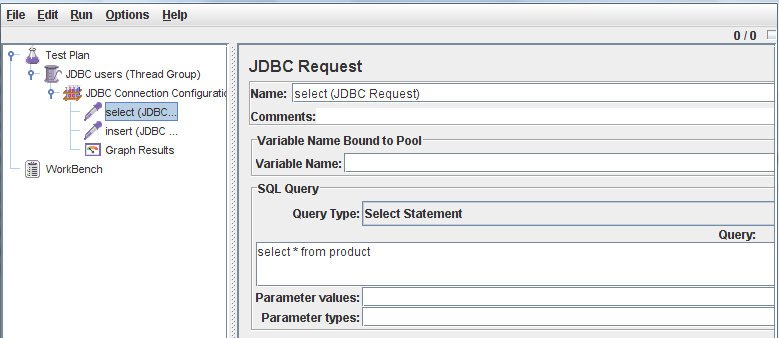
\includegraphics[width=13cm]{img/JMeterSQL.jpg}	
	\end{center}
	\caption{JMeter GUI}
	\label{JMeter}	
\end{figure}

Moreover these load tests can also be executed concurrently by JMeter and in two different ways:
\begin{itemize}
	\item Each thread group can simulate a collection of users with the same behavior. Each user is a thread, and the amount of thread is a parameter of the thread group. Therefore it's possible to simulate different users with the same behavior.
	\item It is also possible to implement different thread groups and so different behavior.
\end{itemize}
The ability to execute load test and concurrent test give us all the flexibility we need to run our test suite, particularly load test case such as the real time prepaid system explained at paragraph \ref{load-test-case}.

Another important feature in favour of JMeter is the capability to load test also databases via JDBC. As already said the figure \ref{JMeter} is an example of a JMeter configuration test for a database via JDBC. It shows how to simulate a group of user with the same behaviour: they firstly execute a select and then an insert. The whole database configuration is setted up by the JDBC Connection Configuration where we need simply to specify the driver to be used and the usual connection parameters, such as the database URL, username and password. 

In figure \ref{JMeter} there is another element which we have not still explained: the Graph Result. JMeter is also capable to represent the results in a graphical form. In figure \ref{JMeterGraph} there is an example of a very simple graph obtained during a database load test (this image is taken from the Apache JMeter tutorial). This Graph Result is only a specific Listener which is possible to configure in the test plan, but there are many other listeners such as Table Result or Monitor Result and so on. It is also possible to execute JMeter from the command line interface, saving precious resources while running the test, logging all the results in a file, and then use a specific application to represent them in better ways.

\begin{figure}[htp!] 
	\begin{center}
		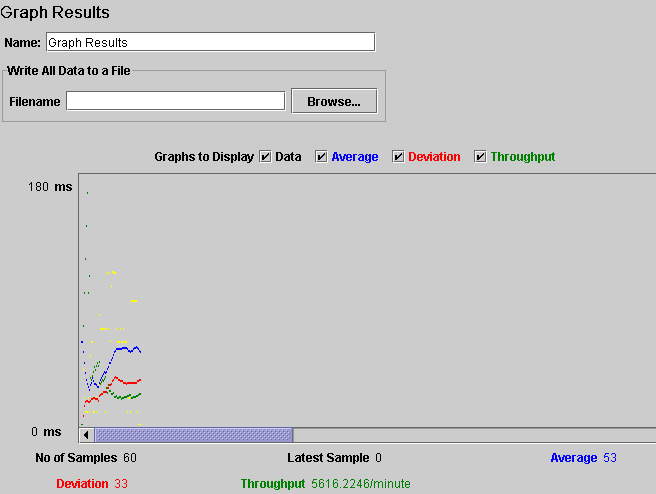
\includegraphics[width=13cm]{img/JMeterGraph.jpg}	
	\end{center}
	\caption{JMeter Graph}
	\label{JMeterGraph}	
\end{figure}

Last but not least, JMeter is based on a plugin architecture and therefore it is highly extensible. Every element can be extended. For example a new Listener with a particular graph can be added, and also new Timers. This feature makes JMeter really flexible, and so another requirement is accomplished.

		\subsection{Disadvantages}
To make this analysis complete, we have also to evaluate the disadvantages of JMeter. And, as first thing, it's evident how JMeter doens't allow load testing of in-memory databases or other kind of databases which don't have a JDBC interface. It only acts with databases through SQL, and it is quite obvious: at the moment there is no a standard for database native interface. Therefore, although JMeter works with relational databases, it will not work with all the in-memory databases without a proper extension, an implementation of a new plugin, because there is no plugin available for our needs.

Moreover JMeter doesn't compare different systems between them, but instead it measures the performance of one system at time. Therefore there is no direct comparison, while the comparison is our main purpose. In fact JMeter was originally designed to test web applications in order to find the best tuning for the web server and the relative application. This means that JMeter is not used to find the best web server with the same application, which in other words it can be said that it is not used to find the best database for our application scenario. Nonetheless it can be also used to compare different systems, but not with much ease of use.

Also the visual representation of the result, the Graph Reult, is not that great, and pf course JMeter is not famouse for graph results. It is not very fluid, and it has some bugs, such as when the test time is too much the graph goes in overflow.

		\subsection{Conclusion}
Now that we have analyzed both advantages and disadvantages...

the graphs are limited

we must implement everything



	
	\section{Poleposition} \label{poleposition}
	Poleposition fa schifo! \cite{poleposition}!!!
	
	\section{Overview's Results}
Tabella riassuntiva, con le caratteristiche di ogni benchmark che ci hanno convinto
Nessun benchmark va bene.
Si potrebbe pensare di prendere alcuni benchmark ed estenderli implementando i casi di nostro interesse.
Oppure fare una nuova applicazione di benchmark...segue nel prossimo capitolo.
	
	
	
	
\chapter{The New In-Memory Database Benchmark Application}
	\section{Functional View}
	\section{Development View}
	\section{Plug-In Architecture}

\chapter{Results' Analysis}
	\section{Why Pico4 is faster}
